%%%%%%%%%%%%%%%%%%%%%%%%%%%%%%%%%%%%%%%%%%%%%%%%%%%%%%%%%%%%%%
%% LaTeX template for the science justification to be       %%
%%       submitted as part of an ALMA proposal.             %%
%%                                                          %%
%%                      ALMA Cycle 3                        %%
%%                                                          %%
%%%%%%%%%%%%%%%%%%%%%%%%%%%%%%%%%%%%%%%%%%%%%%%%%%%%%%%%%%%%%%

%%%%%%%%%%%%%%%%%%%%%%%%%%%%%%%%%%%%%%%%%%%%%%%%%%
%%%%% How to convert this document to PDF %%%%%%%%
%%%%%%%%%%%%%%%%%%%%%%%%%%%%%%%%%%%%%%%%%%%%%%%%%%

% If your figures are stored as PostScript files, you can use the 
% following commands to generate a PDF file of your proposal:

%% latex file.tex
%% dvips file.dvi
%% ps2pdf file.ps file.pdf 


% If your figures are PDF images or bitmap pictures in PNG, JPG, or GIF format,
% you can use the pdflatex command to generate a PDF file from this template
% (note, however, that the pdflatex command does not handle PostScript files):

% pdflatex file.tex


% WARNINGS: 
%           1. You must make sure that PDF output generated from this
%              template is complete both when displayed with a viewer 
%              (acroread, for example) and when printed on paper.
%              LaTeX installations vary greatly and therefore it might 
%              not be possible to get all proposals to come out 
%              correctly with a single text page layout. 
%              In some cases you will have to adjust the 
%              \topmargin=-7mm command in the template to center the 
%              text vertically in the page.  
%           2. The scientific justification, figures, tables, references,
%              and public outreach statement must all fit within the
%              4-page limit.
%           3. You are free to include colour images in your proposal 
%              justification. Proposals are distributed to ALMA Review Panels 
%              in electronic form. However, the scientific content of the 
%              images should still remain clear when displayed or printed
%              in black and white.

%%%%%%%%%%%%%%%%%%%%%%%%%%%%%%%%%%%%%%%%%%%%%%
%%%%% Default format: 12pt single column %%%%%
%% 12pt is the minimum font size allowed !! %%
%%%%%%%%%%%%%%%%%%%%%%%%%%%%%%%%%%%%%%%%%%%%%%

\documentclass[12pt,a4paper]{article}  %% DO NOT CHANGE to 11pt or less !

\usepackage{graphics,graphicx}

%%%%%%%%%%%%%%%%%%%%%%%%%%%%
%%%%%% Page dimensions %%%%%
%%%%%%  DO NOT CHANGE  %%%%%
%%%%%%%%%%%%%%%%%%%%%%%%%%%%

\textheight=247mm
\textwidth=180mm
\topmargin=-7mm
\oddsidemargin=-10mm
\evensidemargin=-10mm
\parindent 10pt

%%%%%%%%%%%%%%%%%%%%%%%%%%%%%
%%%%% Start of document %%%%% 
%%%%%%%%%%%%%%%%%%%%%%%%%%%%%

\begin{document}
\pagestyle{plain}
\pagenumbering{arabic}
 
%%%%%%%%%%%%%%%%%%%%%%%%%%%%%
%%%%% Title of proposal %%%%%
%%%%%%%%%%%%%%%%%%%%%%%%%%%%%

\begin{center}
{\LARGE{\bf
%%
%% ENTER TITLE OF PROPOSAL BELOW THIS LINE
{The most distant galaxies in the universe can be seen by ALMA}
%%
%%
}}
\end{center}
\bigskip

%% Principal Investigator (PI) initial(s) and family name %%
\centerline{\bf PI: 
%% ENTER NAME OF PI BELOW THIS LINE
{Include here the name of the PI}}

\bigskip

% Type a concise abstract of your proposal here (optional).

\section{Abstract}
Include here the abstract of your proposal (optional)

%%%%%%%%%%%%%%%%%%%%%%%%%%%%%%%%%%%%%%%%%
%%%%% Body of science justification %%%%%
%%%%%%%%%%%%%%%%%%%%%%%%%%%%%%%%%%%%%%%%%

%% ENTER TEXT, FIGURES AND TABLES BELOW

\section{Scientific Justification}

Enter the scientific justification here, together with any figures and tables that you judge necessary.
 
%-----------------------------Figure Start---------------------------
\begin{figure}[tbh]
% The 'scale' parameter below allows you to scale the figure so that it fits within the page. In this case the figure was scaled to 20% of its original size. Note: for .png files one has to use pdflatex, not classic latex
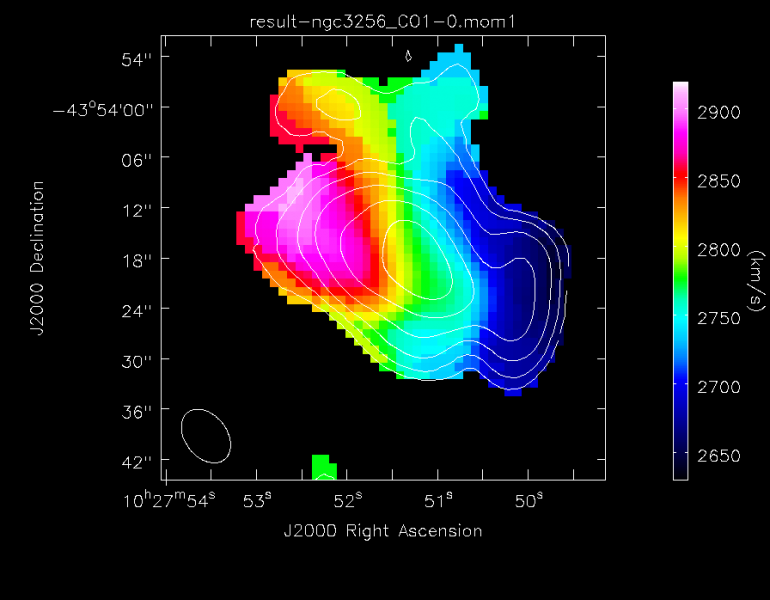
\includegraphics[scale=0.2]{CO_velfield.png}
\caption{\em{The CO(1-0) velocity field of NGC\,3256, with contours 
of the total line emission map overlaid (ALMA Science Verification Data).
}}
\end{figure}
%-----------------------------Figure End------------------------------

%-----------------------------Table Start-----------------------------
\begin{table}[tbh]
\begin{center}
\caption[]{\em{Here we show the continuum sensitivity required per band.}}
\begin{tabular}{cc}
\hline \noalign {\smallskip}
Frequency (GHz) & Sensitivity (mJy) \\
\hline \noalign {\smallskip}
100 & 0.01 \\
300 & 0.10 \\
%\hline \noalign {\smallskip}
\end{tabular}
\end{center}
\end{table}
%-----------------------------Table End ------------------------------

You can structure the scientific justification using the two subsections below (optional).

\subsection{Scientific rationale:}

% Please describe the scientific background of the project,
% pertinent references and previous work relevant to this 
% proposal.

\subsection{Immediate objective:}

% Please describe the observations to be made and their specific
% purpose, with a clear explanation of the need for, and 
% appropriateness of, ALMA Cycle 1 data.  

%%%%%%%%%%%%%%%%%%%%%%%%%%%%%
%% Potential for Publicity %%
%%%%%%%%%%%%%%%%%%%%%%%%%%%%%

\section{Potential for Publicity}

% Here, include a brief statement on the potential of your proposal
% to generate publicity based on the scientific results to be obtained.


%%%%%%%%%%%%%%%%%%%%%%%%
%% References section: %
%%%%%%%%%%%%%%%%%%%%%%%%

\section{References}

% List references here

\noindent [1] Author1 et al. year, journal, vol, page

\noindent [2] Author2 et al. year, journal, vol, page


%%%%%%%%%%%%%%%%%%%%%%%%%%%
%%%%% End of document %%%%%
%%%%%%%%%%%%%%%%%%%%%%%%%%%

\end{document}

